
\chapter{Results}\label{chap:4}
% \section{Prototyping/Evaluating the System}
% 5-7 pages
% \lipsum[1]\todo{TODO}


    
This chapter will provide and overview of the achieved results, th determined baselines, the used data and the experiment process to solve the posed research question. 
This chapter also adapts the structure proposed for machine learning algorithms proposed by \textcite{luckert2016using}.
%  the pipeline deployment details,  collection and labelling steps, the neural network implementation and training. Finally, the pose estimation algorithms and the pipeline are evaluated.
Section \ref{chap:4:setup} illustrates the experiments setup, 
section \ref{chap:4:deployment} describes the deployment of the processing pipeline, 
section \ref{chap:4:train_data} explains the data collection and neural network training, 
% section \ref{chap:4:\ref{chap:4:training}} detailing the training , 
and section \ref{chap:4:results} presents the pipeline results. The following questions will be answered in thoroughly:
\begin{itemize}
    \item What were the experiments setup?
    % \item What was the cloud deployment setup for the solution?
    % \item How many episodes, metrics, etc., were ran and collected for training, testing and optimizing the algorithms?
    \item Which tools were used to acquire the metrics, create the data and perform the experiments?
    % \item Which algorithm parameters were the most influential?
    \item Which algorithm optimizations were done?
    \item What were the achieved results on each experiment?
    % \item What was the setup of the best performing algorithm?
    % \item Which algorithm optimizations were done?
\end{itemize}

\section{Experiment Setup}\label{chap:4:setup}
the experiments were carried out in unity 3D environments

the base experiment environments are
\begin{itemize}
    \item a
    \item b
    \item c
\end{itemize}

the metrics collected were
\begin{itemize}
    \item a
    \item b
    \item c
\end{itemize}

the metrics were collected using bla

the hyperparemeters tuned were
\begin{itemize}
    \item a
    \item b
    \item c
\end{itemize}



    % The design rationale's main concern was to allow for portability and plug-and-play behavior of pose estimation algorithms. We also attempt to minimize assumptions on poses or camera angles (frame information) and account for the natural variation of the cow teats (udder morphology, colors, light conditions, etc.). 
    As proof of concept for the project the test environment that was set up consisted of an artificial cow at the ZHAW and a robotic arm as shown by Figure \ref{fig:cow_setup}. The hardware setup for such an environment consisted of the following:
     \begin{figure}[h]
        \centering
        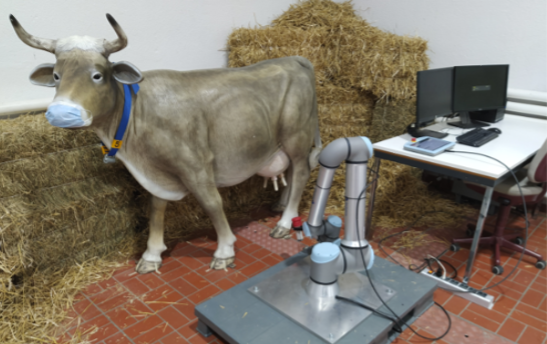
\includegraphics[width=0.7\textwidth]{images/cow_setup.png}
        \caption{Artificial cow setup at the ZHAW}
        \label{fig:cow_setup}
    \end{figure}
    
    \begin{itemize}
        \item \textbf{Blackbox PC:} where the Robot Operating System was running the pose estimation and the robot manipulation.
        \item \textbf{UR10e robot:} industrial robot used in machine tending, palletizing, and packaging (6 axis).
        \item \textbf{Arm Flange:} the flange at the end of the arm had the camera and the milking cup.
        \item \textbf{Dummy cow:} artificial cow model with fake teats to test the robotic attachment.
    \end{itemize}
   
    
    An important aspect in the physical setup for the given task is the specific camera characteristics. A camera can have different performances as a factor to light conditions, shifting, object colors, glass panels and lower resolutions. Given the systemic error a camera can introduce, it is essential to minimize the influence of it. Therefore, a camera evaluation was carried out to compare diverse camera manufacturers and models. Appendix \ref{appendix:camera_evaluation} illustrates the performance of different cameras that were available for evaluation, and presents a clear model that outperforms the rest. 


\section{General Performance}
\begin{itemize}
    \item general interpretation
    \item hyperparameter tuning sensitivity
\end{itemize}

\section{Baselines Performance}


\section{PPO vs SAC}


\section{Discuss Abstraction of the World} (will move to discussion but for continuity)


\section{Multiple-Scenario Performance}


\section{Panoramic Performance}


\section{OpenAI Gym Performance}



% To compare the sample efficiency of PPO and SAC, we run a series of experiments to demonstrate the sample efficiency of PPO. We measure the number of episodes and the number of actions to the state transition in the environment. In addition, we analyze the training speed in our experiments.

% We find that PPO can significantly improve sample efficiency while not being sensitive to hyperparameter tuning and also has a smaller variance than SAC. We show a few sample runs and present numerical results on a robot control task and a grid world navigation task. \ref{chap:4:summary} \ref{chap:5:robots}


% \begin{figure}
% \includegraphics[width=1.0\linewidth]{figs/results-on-robots-tutorial/sacs-performance.pdf}
% \caption{Performance comparison of the PPO, SAC, and a vanilla RL agent.}
% \label{fig:sacs-performance}
% \end{figure}


\newpage
\section{Pipeline Deployment}\label{chap:4:deployment}
The deployment of the components was done using docker compose files to leverage the capabilities of microservices, where every component used behaves as a separate component in the application. The benefit gotten out of microservices is that they are small in size, bounded by their context, independently developed and deployable and they allow for message-based communication%todo ADD REF
. 
% For the deployment of the pipeline on the GPU servers, docker images were built per component (RViz, ROSPlay, ROSTeat, PoseEstimator, etc.). A set of docker compose files was used to control the deployment of the docker containers. 
Figure \ref{fig:cow_docker_topology} shows a sample docker-compose file, which describes the services and the volumes being deployed. In this particular example, Pose Estimator waits for ROSTeat to be succesfully deployed, whereas ROSTeat waits for ROSPlay.

\begin{figure}[h]
    \centering
    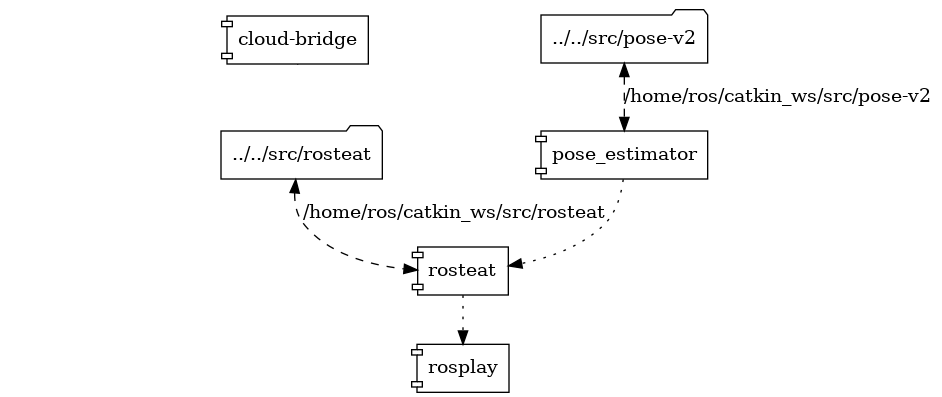
\includegraphics[width=1\textwidth]{images/cow_docker_topology.png}
    \caption{Example of a Docker-compose Deployment}
    \label{fig:cow_docker_topology}
\end{figure}

The components proposed in the previous Chapter were developed both in Python 2.7 and 3.6, which was not an obstacle given the modular approach. The only problem encountered were the outdated packages given that Python 2.7 has been deprecated as of January 1st, 2020. 
Aditionally, the set of libraries and tools used for developing the pose estimation component in the Robot Base was the Robot Operating System (ROS). "ROS provides the services you would expect from an operating system, including hardware abstraction, low-level device control, implementation of commonly-used functionality, message-passing between processes, and package management" \cite{2020ROS}. The specific versions of ROS used for the development were ROS Melodic and ROS Noetic.


\section{Segmentation Network Training}\label{chap:4:train_data}

The training data was collected using the robot's base recording procedure, which stores the set of input frames observed as a video file in ROS format (ROSbag), which could be replayed for future testing or simulations. Rviz can then be used to collect the RGB images and depth images at manually indicated timestamps. The RGB-D input received from the camera consists of images with a resolution of 640 x 480 x 4 pixels. 
% Each pose estimation algorithm receives the input from the camera and the segmentation mask and processes it differently. 
% This was done to analyze the precision from different sources of information (for example, point cloud versus depth image).

\begin{figure}[h]
    \centering
    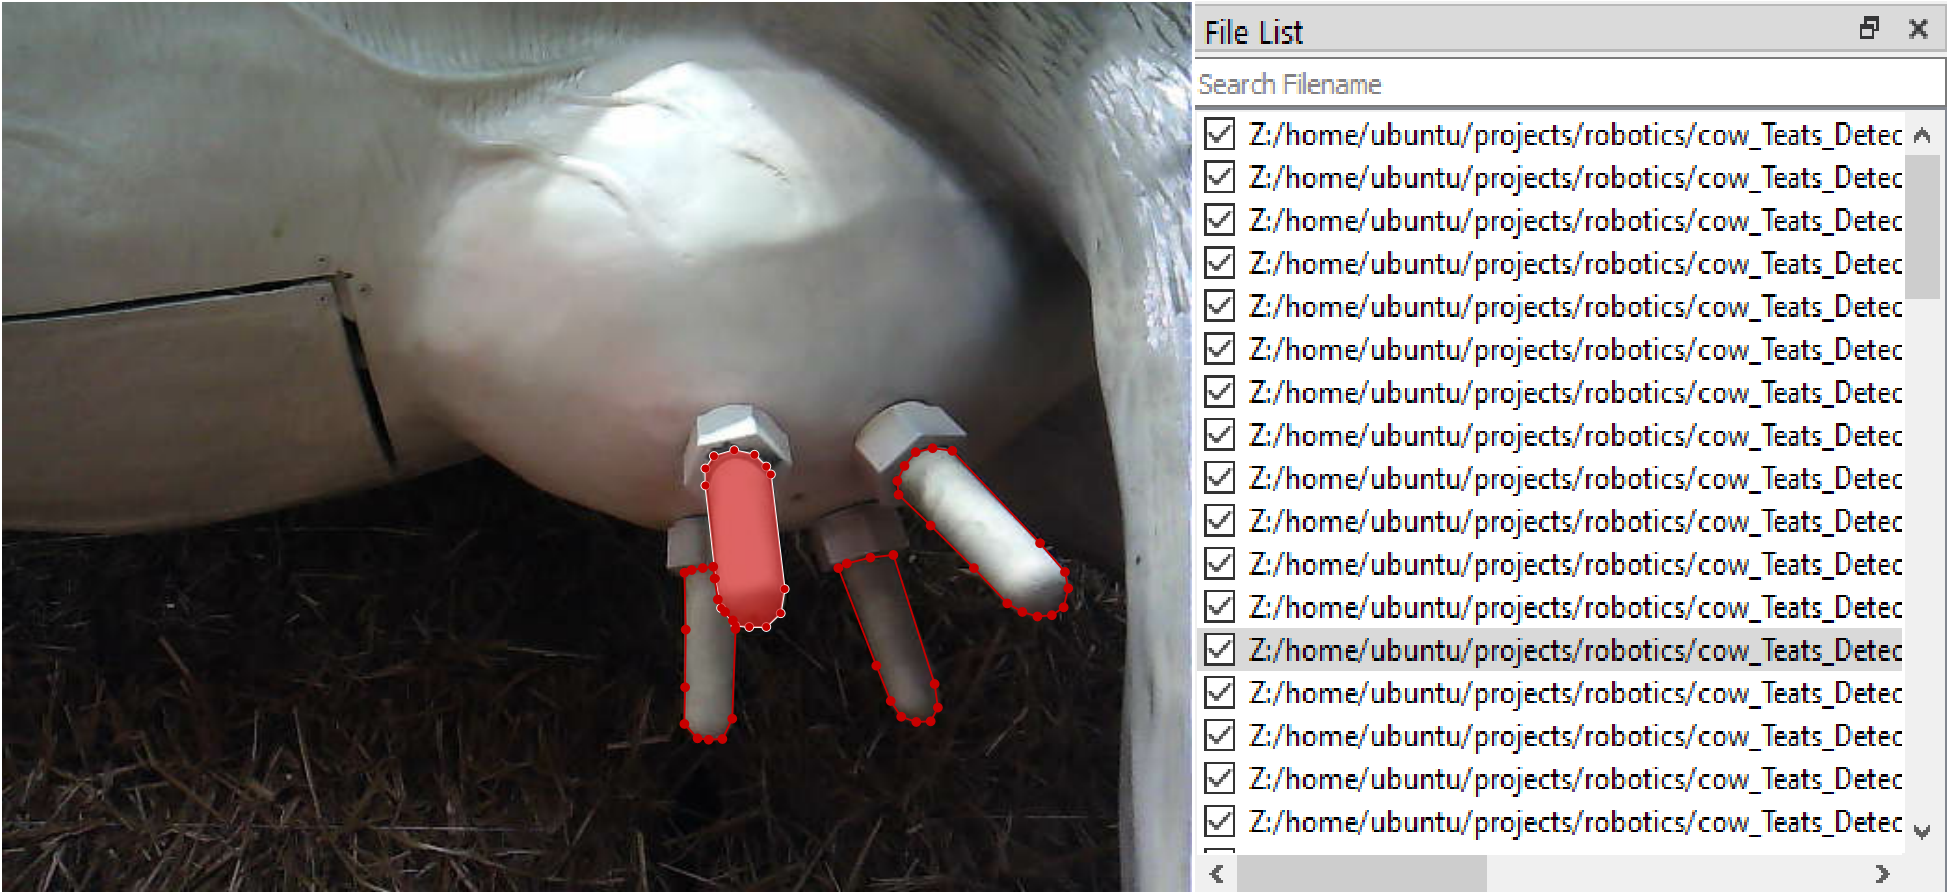
\includegraphics[width=0.4\textwidth]{images/cow_labelme.png}
    \caption{Image annotation example.}
    \label{fig:cow_labelme}
\end{figure}
The collected realistic images are then imported into the image annotation tool LabelMe \cite{2021labelme}. Labelme is used to manually mark the pixel-wise segmentation areas and to assign the class labels.  Figure \ref{fig:cow_labelme} shows a glimpse of the labelling tool. Once an image has been labelled the pixel-wise segmentation is stored as a polygon in JSON file next to the original image. As a final step, a Python script is used to merge all the individual JSON files into one, before feeding the data set into the network for training.

\begin{longtable}{@{} p{8cm} c @{}} \toprule
% \textbf{asd}       & \textbf{Segment Cow Teats from Image} \\ \midrule
Number of Synthetic Training Images generated                   & 400'000 \\ \cmidrule{1-2}
Number of Synthetic Validation Images generated                   & 20'000 \\ \cmidrule{1-2}
Number of Real Training Photos collected             & 192 \\ \cmidrule{1-2}
Number of Real Validation Photos collected             & 192 \\ \cmidrule{1-2}
Total Number of Features                    & 1 \\ \bottomrule
\caption{Data sets statistics.} \label{tab:dataset-statistics} \\
\end{longtable}

The training of MaskRCNN and DOPE was performed on an NVIDIA Tesla T4 GPU \cite{2021testat4}.
% with 16 GB VRAM. 
CUDA \cite{2021nvidia-cuda} was used to parallelize the computations both in training and testing, and therefore speed up the processing times. Table \ref{tab:dataset-statistics} provides an overview of the data set statistics used for training. 
Additionally, the docker images were configured so that the training parameters can be input as environment variables. These parameters include the data set, local weights and the remote weights locations, the epochs, score threshold, learning rate, etc. Table \ref{tab:train-results} show the classification errors of the methods trained

\begin{longtable}{@{} p{5cm} C{2cm}           C{2.5cm}                   C{1.5cm}           C{1.5cm}         @{}} \toprule
\textbf{Method}              & \textbf{Dataset} & \textbf{Learning rate}   & \textbf{Epochs}  & \textbf{Accuracy}  \\ \midrule
matterport/MaskRCNN - Py2.7         & Real        & 0.002                    &  100             & 97\%          \\ \midrule
matterport/MaskRCNN - Py3.6         & Real        & 0.002                    &  100             & 97\%          \\ \midrule
Detectron2/MaskRCNN                 & Real        & 0.00025                  &  2000            & 98\%          \\ \midrule
Detectron2/MaskRCNN                 & Synthetic        & 0.00025                  &  2000            & 0\%          \\ \bottomrule
\caption{Segmentation networks performance.} \label{tab:train-results}
\end{longtable}


As shown above, the synthetic data set proved the images were not photorealistic enough to close the reality gap. Both the matterport and the Detectron2 implementations of MaskRCNN showed similar accuracy. However, the implementation from matterport in Python 2.7 had an initial average loading time of 40 seconds and the implementation in Python 3.6 had a 4 seconds average loading time. Moreover, benchmarks show the implementations from matterport have a 4x slower throughput (imgs/sec) compared to Detectron2 \cite{2021detectron2-benchmark}. These drawbacks and the generally better performance of the Detectron2 implementation led to it being chosen for the segmentation task. 
% Finally, the increase of the prediction score threshold was the only optimization done, other than the parameters shown in Table \ref{tab:train-results}.



\section{Results} \label{chap:4:results}
\subsection{Research Question}
\label{sec:results-research-question}
% \lipsum[1-4]

The research question tackles the pose estimation of cow teats. This section will describe the results obtained for each approach proposed, along with their respective optimizations. 

Table \ref{tab:test-results} provides a brief summary of the results and the general performance of the used algorithms, which are discussed afterwards in more detail.

\begin{longtable}
{@{} l c c @{}} \toprule
\textbf{Method}                     & \textbf{Accuracy}     & \textbf{Standard Deviation}       \\ \midrule
% PCA                                 & 97\%                  & 0.015                             \\ \midrule
MAV                                 & \textbf{97\% }                 & \textbf{0.43}                             \\ \midrule
DOPE                                & 0\%                  & -                             \\ \midrule
RANSAC                              & 0\%                   & -                             \\ \bottomrule
\caption{Statistics of tested methods.} \label{tab:test-results}                          \\
\end{longtable}

% The following Table displays the results for the PCA-variant algorithm. The variants presented are optimized by modifying the offset and the averaging mechanism used to calculate the Teat Tip coordinates.
% \begin{longtable}{|p{1.5cm}|p{3cm}|C{1.5cm}|}                                              \hline
% \multicolumn{3}{|l|}{\textbf{PCA-variant}}                                                       \\\hline
% \textbf{Offset}         & \textbf{Averaging Method}   & \textbf{Accuracy}                \\ \hline
% Fixed                   & Single Point                & 97\%                             \\ \hline
% Mixed                   & Single Point                & 97\%                             \\ \hline
% Fixed                   & Average: 1/3rd              & 97\%                             \\ \hline
% Mixed                   & Average: 1/10th             & 97\%                             \\ \hline
% \caption{Overview of the best MAV results for the respective offset-averaging mechanisms combinations.} \label{tab:test-results}                          
% \end{longtable}

% The following Table displays the results for the Normals algorithm. The variants presented are optimized by modifying the offset and the averaging mechanism used to calculate the Teat Tip coordinates.
% \begin{longtable}{|p{1.5cm}|p{3cm}|C{1.5cm}|}                                              \hline
% \multicolumn{3}{|l|}{\textbf{Normals}}                                                       \\\hline
% \textbf{Offset}         & \textbf{Averaging Method}   & \textbf{Accuracy}                \\ \hline
% Fixed                   & Single Point                & 97\%                             \\ \hline
% Mixed                   & Single Point                & 97\%                             \\ \hline
% Fixed                   & Average: 1/3rd              & 97\%                             \\ \hline
% Mixed                   & Average: 1/10th             & 97\%                             \\ \hline
% \caption{Overview of the best MAV results for the respective offset-averaging mechanisms combinations.} \label{tab:test-results}                          
% \end{longtable}

The following Table \ref{tab:DOPE-results} displays the results for the DOPE algorithm. DOPE uses FAT formatted data sets, which are generated using NDDS, in Unreal Engine 4. These data sets are characterized for being synthetic photorealistic images. The data set variants presented below are optimized by modifying the parameters in data set used, such as:
% The variants used include changes in: 
the realism degree in the materials used for the object textures, the usage of rotation in the focus object, and the usage of obstructive objects. Aditionally, all data sets include five different photorealistic scenes: beach, studio, temple, meadow and zen garden. Surprisingly none of the data sets were realistic enough to close the reality gap, which reflected in DOPE not outputting any predictions.

\begin{longtable}{|l|c||c|}                            \hline
\multicolumn{3}{|l|}{\textbf{Deep Object Pose}}              \\\hline
\textbf{Dataset}            & \textbf{Size}  & \textbf{Functional}            \\ \hline
NDDS Photorealistic (base)       & 260k      & No                             \\ \hline
NDDS Photorealistic 2.0          & 80k       & No                             \\ \hline
NDDS with Obstruction       & 80k       & No                             \\ \hline
NDDS with Rotation          & 80k       & No                             \\ \hline
NDDS Small                  & 20k       & No                             \\ \hline
\caption{Overview of the best DOPE results for the respective dataset variations.} \label{tab:DOPE-results}
\end{longtable}

The results for the RANSAC algorithm are shown in Table \ref{tab:ransac-results}. The skimage implementation was used for both RANSAC and direct ORB matching. The variants presented were surprinsingly not succesful at matching the cow teats patterns. It is suspected that RANSAC and ORB matching are not the best approach for identifying simple texture objects such as the cow teats. 
Figure \ref{fig:ransac-results} illustrates the suspicion and the behavior of RANSAC on both the RGB and the depth images. RANSAC was tested by varying the ORB number of keypoints, the ORB threshold and RANSAC's residual threshold as well as adding a denoising step.  
% \begin{longtable}{|p{1.5cm}|p{3cm}|C{1.5cm}|}                                              \hline
% \multicolumn{3}{|l|}{\textbf{RANSAC}}                                                       \\\hline
% \textbf{Offset}         & \textbf{Averaging Method}   & \textbf{Functional}                \\ \hline
% Fixed                   & Single Point                & No\%                             \\ \hline
% Mixed                   & Single Point                & No\%                             \\ \hline
% Fixed                   & Average: 1/3rd              & No\%                             \\ \hline
% Mixed                   & Average: 1/10th             & No\%                             \\ \hline
% \caption{Overview of the best MAV results for the respective offset-averaging mechanisms combinations.} \label{tab:test-results}                          
% \end{longtable}
\begin{longtable}{|c|c|c|c||c|}                            \hline
\multicolumn{5}{|l|}{\textbf{RANSAC / ORB Matching}}              \\\hline
\textbf{ORB \#keypoints} & \textbf{ORB threshold} & \textbf{Residual Threshold} & \textbf{Denoising}       & \textbf{Functional}      \\ \hline
        20      & 0.08      & N/A (ORB matching)       & No     &  No               \\ \hline
        200     & 0.08      & N/A (ORB matching)       & No     &  No               \\ \hline
        200     & 0.02      & 0.5       & No     &  No               \\ \hline
        200     & 0.02      & 0.5       & Yes    &  No               \\ \hline
        200     & 0.02      & 0.9       & No     &  No               \\ \hline
        200     & 0.02      & 0.9       & Yes    &  No               \\ \hline
        200     & 0.08      & 0.5       & No     &  No               \\ \hline
        200     & 0.08      & 0.5       & Yes    &  No               \\ \hline
        200     & 0.08      & 0.9       & No     &  No               \\ \hline
        200     & 0.08      & 0.9       & Yes    &  No               \\ \hline
\caption{Overview of the best MAV results for the respective offset-averaging mechanisms combinations.} \label{tab:ransac-results}                          
\end{longtable}

 \begin{figure}[h]
        \centering
        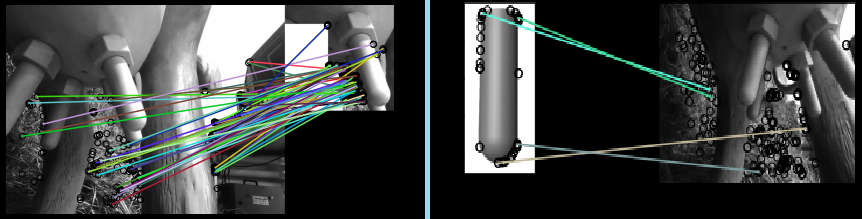
\includegraphics[width=0.9\textwidth]{images/cow_ransac.png}
        \caption{RANSAC's behavior on the cow data set.}
        \label{fig:ransac-results}
    \end{figure}
    
The following table 
% \ref{tab:mav-results} displays 
presents the results for the "MAV" algorithm. The optimizations presented are a combination of the offset and the averaging method.

\begin{longtable}{|l|l||c|c|c|}                                              \hline
\multicolumn{5}{|l|}{\textbf{MAV}}                                                       \\\hline
\textbf{Offset}         & \textbf{Averaging Method}   
& \textbf{Average Error}  & \textbf{Standard Deviation}  & \textbf{Execution Time}                 \\ \hline
Fixed                   & Single Point                & 1.13            & 2.8              & 0.26 - 1.5 secs   \\ \hline
Calculated              & Single Point                & 1.77            & 3.3              & 0.26 - 1.5 secs   \\ \hline
Fixed                   & Average: 1/3rd              & \textbf{0.67}   & \textbf{2.4}     & 0.26 - 1.5 secs                     \\ \hline
Calculated              & Average: 1/3rd              & 1.54            & 2.93             & 0.26 - 1.5 secs    \\ \hline
Fixed                   & Average: 1/10th             & 0.96            & 2.55             & 0.26 - 1.5 secs     \\ \hline
Calculated              & Average: 1/10th             & 1.51            & 2.87             & 0.26 - 1.5 secs    \\ \hline
\caption{Overview of the best MAV results for the respective offset-averaging mechanisms combinations.} \label{tab:mav-results}                          
\end{longtable}

% \subsection{Research Question 2}

% The second research question tackles the evaluation of the pose estimation of cow teats.

% \subsection{Quality Ranking of Predictions}
\subsection{Deliverables}
The following deliverables will be handled in with this Vertiefungsarbeit:
\begin{itemize}
    \item This work produced a pose estimation system, which is able to estimate a cow teat's pose with an average error of 0.67 cm and a standard deviation of 2.4 cm. 
    \item This work also contributed to two other successful alternatives to the MAV algorithm that were developed by the project team for the cow teats project.
    \item For future research, an Unreal Engine 4 project with 5 different photorealistic scenes for a synthetic data set generation, including a cow teats data set containing over 400,000 images for pose estimation.
\end{itemize}